% Copyright (c) 2022 Tobias Briones. All rights reserved.
%
% SPDX-License-Identifier: CC-BY-SA-4.0
%
% This file is part of Course Project at UNAH-IS911: Microprocessors.
%
% This source code is licensed under the Creative Commons Attribution Share
% Alike 4.0 International License found in the LICENSE file in the root
% directory of this source tree or at https://spdx.org/licenses/CC-BY-SA-4.0.

\documentclass{article}
\usepackage[letterpaper, portrait, margin=2cm]{geometry}
\usepackage[style=ieee]{biblatex}
\usepackage[utf8]{inputenc}
\usepackage[spanish]{babel}
\usepackage{geometry}
\usepackage[]{graphics}
\usepackage[demo]{graphicx}
\usepackage{csquotes}
\usepackage{float}
\usepackage{hyperref}
\usepackage[table,xcdraw]{xcolor}
\usepackage{lipsum}
\usepackage{listings}
\usepackage{dirtytalk}


\addbibresource{bibliography.bib}

\hypersetup{
    colorlinks=true,
    linkcolor=black,
    filecolor=magenta,
    urlcolor=cyan,
    citecolor=black
}

\definecolor{codegreen}{rgb}{0,0.6,0}
\definecolor{codegray}{rgb}{0.5,0.5,0.5}
\definecolor{codepurple}{rgb}{0.58,0,0.82}
\definecolor{backcolour}{rgb}{0.95,0.95,0.92}

\lstdefinestyle{mystyle}{
    commentstyle=\color{codegreen},
    keywordstyle=\color{magenta},
    numberstyle=\tiny\color{codegray},
    stringstyle=\color{codepurple},
    basicstyle=\ttfamily\footnotesize,
    breakatwhitespace=false,
    breaklines=true,
    captionpos=b,
    keepspaces=true,
    numbers=left,
    numbersep=5pt,
    showspaces=false,
    showstringspaces=false,
    showtabs=false,
    tabsize=2
}

\lstset{style=mystyle}

\newcommand\blfootnote[1]{
    \begingroup
    \renewcommand\thefootnote{}\footnote{#1}
    \addtocounter{footnote}{-1}
    \endgroup
}

\title{LAB 3: CONFIGURANDO UN LCD}
\author{Tobias Briones \bigbreak tobias.briones@unah.hn}
\date{\today}

\begin{document}

    \makeatletter
    \begin{titlepage}
        \begin{center}
            
\includegraphics[width=0.3\linewidth]{images/logo-unah.png}\\[4ex]
            {\huge \bfseries \@title
            \vspace{1cm}}\\[2ex]
            {\LARGE \@author}\\[50ex]

            {\large
            Universidad Nacional Autónoma de Honduras\\
            Ingeniería de Sistemas\\
            I PAC 2022\\
            IS911-MICROPROCESADORES
            }\\[2ex]

            {\large \today}
        \end{center}
    \end{titlepage}
    \makeatother
    \thispagestyle{empty}
    \newpage

    \blfootnote{
        Copyright (c) 2022 Tobias Briones. All rights reserved. \\
        This work is licensed under the Creative Commons Attribution Share Alike 4.0 International License (\href{https://spdx.org/licenses/CC-BY-SA-4.0}{CC-BY-SA-4.0}). \\
        Third party contents available under their respective copyright and license.\\
        For more details go to the \href{https://github.com/tobiasbriones/cp-unah-is911-microprocessors}{GitHub Repository}.}

    \section{Objetivo}

    Desarrollar un projecto en Arduino y Proteus para imprimir una cadena de texto por un LCD.

    \subsection{Objetivos Específicos}

    \begin{itemize}
        \item Desarrollar el programa Arduino.
        \item Establecer el circuito para el LCD.
        \item Crear y correr la simulación del proyecto en Proteus.
    \end{itemize}

    \section{Marco Teórico}

    LCD significa $Liquid Crystal Display$ y son pantallas muy populares para hacer proyectos en Arduino. Estas cuentan con un arreglo de rejilla y se diferencian en tamaño por la cantidad de columnas y filas que tienen. El texto se puede imprimir y actualizar en la pantalla mediante Arduino o cualquier microcontrolador como un PIC y también se pueden enviar otros comandos al LCD y manejar la cantidad de contraste que tenga la pantalla.

    \begin{figure}[H]
        \centering
        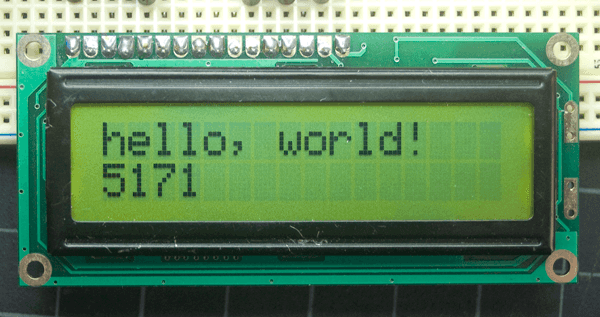
\includegraphics[width=0.3\paperwidth]{images/lcd-photo.png}
        \caption{LCD de 16x2}\footnotesize
        Fuente: \textit{Arduino Docs $\mid$ Liquid Crystal Displays (LCD) with Arduino}. Licensed under the Creative Commons Attribution-Share Alike 4.0 License. \cite{arduino-docs-lcd-2021}
    \end{figure}

    Los LCDs trabajan con interfase en paralelo por lo que hay que configurar varios pines para controlar la pantalla y los pines que se utilizan consisten en \cite{arduino-docs-lcd-2021}:

    \begin{itemize}
        \item \textbf{El selector de registro (RS):} Controla las acciones a tomar para el LCD ya sea para imprimir texto o comandos para instrucciones para el LCD.
        \item \textbf{Lectura/Escritura (RW):} Configura el modo como lectura o escritura.
        \item \textbf{Habilitador:} Este pin habilita la escritura para los registros.
        \item \textbf{8 pines de datos $D_0-D_7$:} Los valores digitales de estos pines son los que ya sea se escriben o leen.
    \end{itemize}

    Por último también está el pin para configurar el contraste $V_0$, el de alimentación que requiere $5V$, y el tierra.

    \subsection{Bus I2C}

    I2C es un protocolo que usa solo dos líneas para enviar y recibir datos: reloh (SCL) y datos (SDA). Cada bit forma una sucesión que da la dirección de un dispositivo y un dato o comando que son mandados por el pin SDA. El dispositivo puede también responder de vuelta hacia el Arduino \cite{arduino-docs-i2c-2021}.

    \section{Procedimiento Experimental}

    Para conectar un LCD al Arduino se utilizará la biblioteca $LiquidCrystal$ que trae ya el Arduino IDE. Para hacer la conexión del LCD es posible hacerlo directamente como se ha descrito o instalar de internet una biblioteca que extiende a la mencionada y que permite usar un bus I2C de forma que solo se necesitan $2$ pines para establecer la conexión con la tarjeta Arduino. Esto requiere algunos pasos extras y que se dejan al lector para su exploración.

    \bigbreak

    El programa consiste en el siguiente snippet:

    \begin{lstlisting}[language=C, caption=Arduino Sketch]
#include <LiquidCrystal.h>

LiquidCrystal lcd(7, 8, 9, 10, 11, 12);

void setup() {
  lcd.begin(16, 2);
  lcd.setCursor(4, 1);
  lcd.write("IES ZOCO");
}

void loop() {}
    \end{lstlisting}

    \begin{figure}[H]
        \centering
        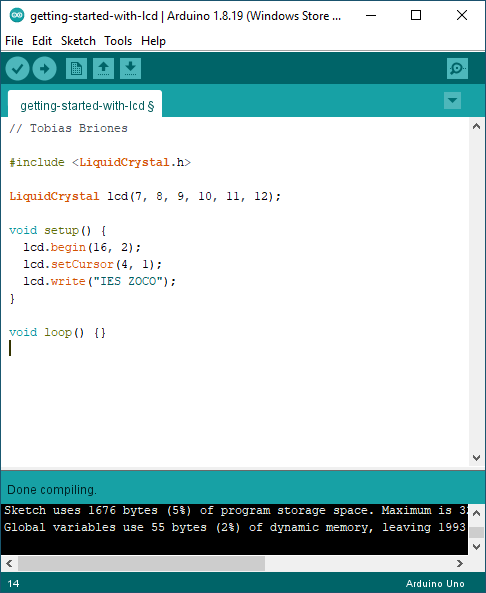
\includegraphics[width=0.3\paperwidth]{images/arduino-sketch.png}
        \caption{Programa Arduino para configuración del LCD}\footnotesize
        \textit{Derivative screenshot from Arduino IDE under fair use}
    \end{figure}

    El código es super sencillo pero hay que tener en cuenta los argumentos para el objeto $LiquidCrystal$. Para empezar se importa la biblioteca $LiquidCrystal$ y se instancia un objeto $LiquidCrystal$ para manejar el LCD. En el $setup$ se configura al LCD como una rejilla de $16$ columnas por $2$ filas, se pone el cursor en la posición $4 \, 1$ y se escribe el texto deseado \say{IES ZOCO} por ejemplo. En el loop del programa no se hará ninguna actualización.

    \bigbreak

    La firma del constructor $LiquidCrystal$ es:

    $$LiquidCrystal lcd(rs, en, d_4, d_5, d_6, d_7);$$

    donde $rs$ es el selector de registro y $en$ es habilitar. Los otros $4$ pines son los datos para imprimir el texto.

    \bigbreak

    Ahora hay que fijarse en el diagrama del circuito.

    \begin{figure}[H]
        \centering
        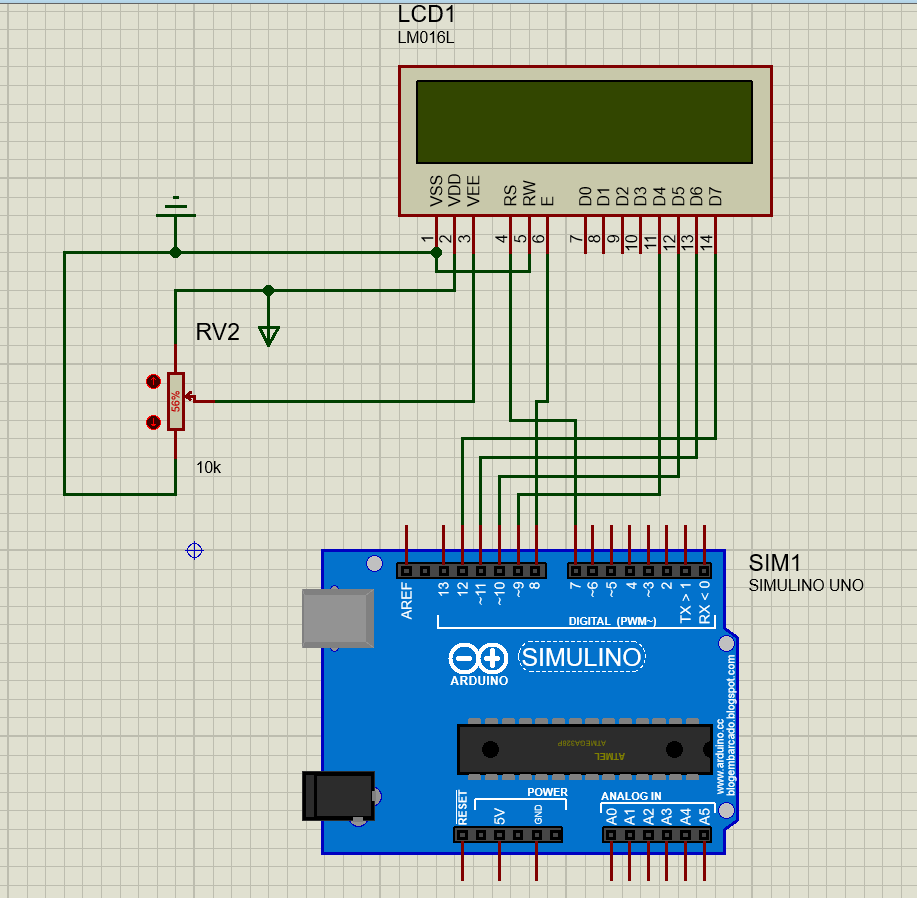
\includegraphics[width=0.6\paperwidth]{images/sim-schematic.png}
        \caption{Diagrama del circuito para configuración del LCD}\footnotesize
        \textit{Derivative screenshot from Proteus under fair use}
    \end{figure}

    Se debe conectar $VSS$ y $RW$ a tierra. $RW$ va a tierra ya que se quiere mantener enviando caracteres de forma constante y no se mandarán comandos diferentes. $VDD$ va a alimentación y $VEE$ va al potenciómentro de $10K$ para controlar el contraste del LCD el cual es un divisor de tensión para esa terminal. $RS$ se conecta al pin $7$ y $E$ (enable) al $8$. Los bits del $D_0$ al $D_3$ no se usarán y se establecerá la conexión con los otros cuatro bits restantes $D_4-D_7$.

    \bigbreak

    Los dispositivos necesarios son simplemente:

    \begin{figure}[H]
        \centering
        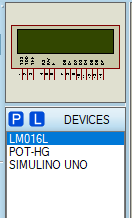
\includegraphics[width=0.2\paperwidth]{images/sim-devices.png}
        \caption{Dispositivos necesarios para el programa del LCD}\footnotesize
        \textit{Derivative screenshot from Proteus under fair use}
    \end{figure}

    \bigbreak

    Al correr la simulación se obtiene un resultado como el siguiente:

    \begin{figure}[H]
        \centering
        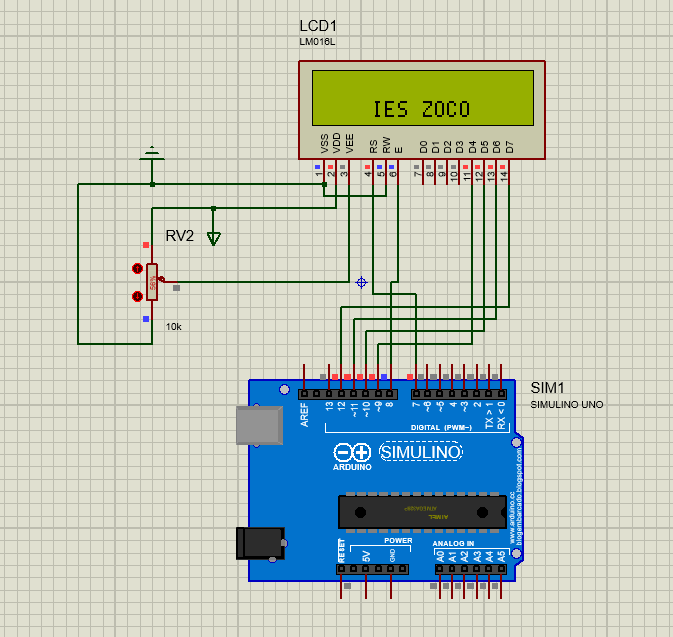
\includegraphics[width=0.6\paperwidth]{images/sim-running.png}
        \caption{Simulación del programa para el LCD}\footnotesize
        \textit{Derivative screenshot from Proteus under fair use}
    \end{figure}

    \section{Análisis de Resultados}

    Al correr la simulación se imprimió inmediatamente el texto dado en la pantalla del LCD tal como se configuró en la rejilla del LCD utilizado.

    \bigbreak

    Al hacer variar el potenciómetro se pudo manejar el contraste del LCD de menor a mayor valor.

    \section{Conclusión}

    Se desarrolló un programa en Arduino que configura de forma básica un LCD que se implementó con el circuito correspondiente en Proteus y se corrió la simulación obteniendo el resultado esperado para establecer la conexión del LCD con la tarjeta Arduino.

    \printbibliography

\end{document}
